% context: 9th-grade physics classwork, Unit 2 kinematics, Giancoli 2-8 (pp. 38-40)
% topic: graphs of free fall; a dropped stone's table at 0.5 s steps (as in 2-5CW Q1
%        and 2-5HW Q10), y vs t is half a parabola, v vs t is a straight line whose
%        slope is g; chord slope = average velocity, tangent slope = instantaneous
%        velocity (2-2CW Q4); a ball thrown upward: the top of the parabola is where
%        the tangent is flat and v = 0
% structure: two pages; page 1 the table and both graphs to plot, side by side;
%        page 2 chords and a tangent on the page-1 position graph, then reading a
%        given graph of a ball thrown up and sketching its velocity graph. Students may not finish the plotting in
%        class, which is fine
% data: g is rounded to 10 m/s^2 so the points land on grid lines (y = 5t^2) and the
%        squares of 0.5, 1.5, 2.5 practise the 2-6DN decimal-squaring error
\documentclass[12pt, twoside]{article}
%\documentclass[12pt, twoside]{article}
\usepackage[letterpaper, margin=1in, headsep=0.2in]{geometry}
\setlength{\headheight}{0.6in}
%\usepackage[english]{babel}
\usepackage[utf8]{inputenc}
\usepackage{microtype}
\usepackage{amsmath}
\usepackage{amssymb}
%\usepackage{amsfonts}
\usepackage[nomessages]{fp} %\FPeval{\var-name}{2*sin(pi/6)}
\usepackage{siunitx} %units in math. eg 20\milli\meter
\usepackage{yhmath} % for arcs, overparenth command
\usepackage{tikz} %graphics
\usetikzlibrary{quotes, angles, arrows, arrows.meta}
\usepackage{graphicx} %consider setting \graphicspath{{images/}}
\usepackage{parskip} %no paragraph indent
\usepackage{enumitem}
\usepackage{multicol}
\usepackage{venndiagram}

\usepackage{fancyhdr}
\pagestyle{fancy}
\fancyhf{}
\renewcommand{\headrulewidth}{0pt} % disable the underline of the header
\raggedbottom
\hfuzz=2mm %suppresses overfull box warnings

\usepackage{hyperref}
\usepackage{float}

\title{Physics}
\author{Chris Huson}
\date{November 2026}

\fancyhead[LE]{\thepage}
\fancyhead[RO]{\thepage \\ Nickname: \hspace{2.25cm} \,\\ \,}
\fancyhead[LO]{La Scuola d'Italia / Huson / Physics \\* 12 November 2026}

\begin{document}

\subsubsection*{2.7 Classwork: Graphing Free Fall}

\textbf{Reference (provided).} \quad A stone is dropped from rest. Take \emph{down} as
positive, with $y_0 = 0$. Then \quad $v = gt$ \quad and \quad $y = \frac{1}{2}gt^2$.

For graphing, round $g$ to 10 m/s$^2$, so $v = 10\,t$ and $y = 5\,t^2$.

\vspace{0.1cm}

\begin{enumerate}[itemsep=0.4cm]

\item Fill in the table. Square the time first: $0.5^2 = 0.25$, so at 0.5 s,
  $y = 5 \times 0.25 = 1.25$ m.

  \vspace{0.1cm}
  {\renewcommand{\arraystretch}{1.5}%
  \begin{tabular}{| l | p{1.15cm} | p{1.15cm} | p{1.15cm} | p{1.15cm} | p{1.15cm} |
      p{1.15cm} | p{1.15cm} |}
    \hline
    $t$ (s) & \centering 0 & \centering 0.5 & \centering 1.0 & \centering 1.5 &
      \centering 2.0 & \centering 2.5 & \centering\arraybackslash 3.0 \\ \hline
    $v$ (m/s) & & & & & & & \\ \hline
    $y$ (m) & & 1.25 & & & & & \\ \hline
  \end{tabular}}

\item \textbf{Graphs.} Plot $y$ against $t$ on the position grid, and join the
  points with a smooth curve, not with straight segments. Plot $v$ against $t$ on the
  velocity grid, and join the points with a ruler.

  \begin{tikzpicture}[x=1.95cm, y=0.135cm]
    \draw[gray!25, thin, xstep=0.1, ystep=1] (0,0) grid (3,45);
    \draw[gray!60, xstep=0.5, ystep=5] (0,0) grid (3,45);
    \draw[->, thick] (0,0) -- (3.12,0) node[below right]{\small $t$ (s)};
    \draw[->, thick] (0,0) -- (0,47.5) node[above]{\small $y$ (m)};
    \foreach \t in {0,0.5,1.0,1.5,2.0,2.5,3.0} \node[below] at (\t,0) {\scriptsize \t};
    \foreach \y in {5,10,...,45} \node[left] at (0,\y) {\scriptsize \y};
    \node[above] at (1.5,47.5) {\small Position};
    % Solution curve — uncomment to see the answer
    %\draw[very thick, domain=0:3, samples=60] plot (\x, {5*\x*\x});
    %\foreach \t in {0,0.5,1,1.5,2,2.5,3} \fill (\t, {5*\t*\t}) circle (1.5pt);
  \end{tikzpicture}
  \hfill
  \begin{tikzpicture}[x=1.95cm, y=0.2025cm]
    \draw[gray!25, thin, xstep=0.1, ystep=1] (0,0) grid (3,30);
    \draw[gray!60, xstep=0.5, ystep=5] (0,0) grid (3,30);
    \draw[->, thick] (0,0) -- (3.12,0) node[below right]{\small $t$ (s)};
    \draw[->, thick] (0,0) -- (0,31.7) node[above]{\small $v$ (m/s)};
    \foreach \t in {0,0.5,1.0,1.5,2.0,2.5,3.0} \node[below] at (\t,0) {\scriptsize \t};
    \foreach \v in {5,10,...,30} \node[left] at (0,\v) {\scriptsize \v};
    \node[above] at (1.5,31.7) {\small Velocity};
    % Solution line — uncomment to see the answer
    %\draw[very thick] (0,0) -- (3,30);
    %\foreach \t in {0,0.5,1,1.5,2,2.5,3} \fill (\t, {10*\t}) circle (1.5pt);
  \end{tikzpicture}

  \begin{enumerate}[itemsep=1.1cm]
    \item Is the position graph a straight line? What does it mean that the curve
      gets steeper and steeper?
    \item At $t = 0$ the position graph is flat. Why?
    \item Find the slope of the velocity graph. Use two points far apart, and give
      the units. What quantity is the slope?
  \end{enumerate}

\newpage

\item \textbf{Chords and a tangent.} Work on your position graph. As with the cart in
  2.2, the slope of a chord is an \emph{average} velocity, and the slope of the
  tangent is the \emph{instantaneous} velocity.
  \begin{enumerate}[itemsep=0.6cm]
    \item Draw the chord joining the points at $t = 1.0$ s and $t = 2.0$ s. Find its
      slope, $\Delta y / \Delta t$. This is the average velocity from 1.0 s to 2.0 s.
    \item Draw the chord from $t = 1.0$ s to $t = 1.5$ s, and find its slope.
    \item Read the velocity at $t = 1.0$ s from your velocity graph. As the chord
      gets shorter, its slope gets closer to this value. Draw the tangent at
      $t = 1.0$ s: the straight line through (1.0 s, 5 m) with this slope.
    \item The average velocity from 1.0 s to 2.0 s, in (a), equals the velocity at
      one moment. Use your velocity graph to find when.
  \end{enumerate}

  \vspace{0.6cm}

\item A ball is thrown straight up at 15 m/s. Take \emph{up} as positive. The left
  graph shows its height above the hand.

  \vspace{0.1cm}
  \begin{tikzpicture}[x=1.95cm, y=0.32cm]
    \draw[gray!25, thin, xstep=0.1, ystep=0.5] (0,0) grid (3,12);
    \draw[gray!60, xstep=0.5, ystep=2] (0,0) grid (3,12);
    \draw[->, thick] (0,0) -- (3.12,0) node[below right]{\small $t$ (s)};
    \draw[->, thick] (0,0) -- (0,13) node[above]{\small $y$ (m)};
    \foreach \t in {0,0.5,1.0,1.5,2.0,2.5,3.0} \node[below] at (\t,0) {\scriptsize \t};
    \foreach \y in {2,4,...,12} \node[left] at (0,\y) {\scriptsize \y};
    \draw[very thick, domain=0:3, samples=60] plot (\x, {15*\x - 5*\x*\x});
  \end{tikzpicture}
  \hfill
  \begin{tikzpicture}[x=1.95cm, y=0.128cm]
    \draw[gray!25, thin, xstep=0.1, ystep=1] (0,-15) grid (3,15);
    \draw[gray!60, xstep=0.5, ystep=5] (0,-15) grid (3,15);
    \draw[->, thick] (0,0) -- (3.12,0) node[above right]{\small $t$ (s)};
    \draw[->, thick] (0,-15) -- (0,16.5) node[above]{\small $v$ (m/s)};
    \foreach \t in {0.5,1.0,1.5,2.0,2.5,3.0}
      \node[below, fill=white, inner sep=1pt] at (\t,-0.4) {\scriptsize \t};
    \foreach \v in {-15,-10,...,15} \node[left] at (0,\v) {\scriptsize \v};
    % Solution line — uncomment to see the answer
    %\draw[very thick] (0,15) -- (3,-15);
  \end{tikzpicture}

  \begin{enumerate}[itemsep=0.7cm]
    \item When is the ball highest, and how high does it go?
    \item What is the slope of the tangent at the top? So what is the ball's
      velocity there?
    \item Where is the slope of the height graph positive, and where is it negative?
      What is the ball doing in each part?
    \item Sketch the velocity graph on the right-hand grid. It starts at $+15$ m/s
      and loses 10 m/s every second. When does it cross zero?
  \end{enumerate}

\end{enumerate}
\end{document}
